% TraceAssist architecture for traceassist_report.tex: tmll_extended_architecture.tex with the
% AI skills (thread_finder, match_judge, view_picker) and the thread search added.
% TMLL architecture extended with this project's additions. Layout and palette
% follow Fig. 2 of tmll/tmll_researchpaper.pdf; boxes tagged NEW were added in
% this project. Standalone; build with
%   pdflatex tmll_extended_architecture.tex
% and include with \includegraphics[width=\textwidth]{tmll_extended_architecture}.
\documentclass[tikz,border=3mm]{standalone}
\usepackage[T1]{fontenc}
\usepackage[scaled=0.92]{helvet}
\renewcommand{\familydefault}{\sfdefault}
\usetikzlibrary{arrows.meta,calc,backgrounds,shadows}

% Palette sampled from the original figure.
\definecolor{user}{HTML}{8579AE}
\definecolor{client}{HTML}{A86E73}
\definecolor{blue}{HTML}{7EA6E0}
\definecolor{green}{HTML}{67AB9F}
\definecolor{mlchip}{HTML}{E59A97}
\definecolor{tsp}{HTML}{A6977F}
\definecolor{server}{HTML}{EA6B66}
\definecolor{results}{HTML}{FFB570}
\definecolor{panel}{HTML}{EEEEEE}
\definecolor{line}{HTML}{6E6E6E}
\definecolor{findings}{HTML}{D9984F}
\definecolor{service}{HTML}{5B7DB1}
\definecolor{badge}{HTML}{2F3B4C}

\newcommand{\sub}[1]{{\fontsize{6.6}{7.8}\selectfont #1}}

\begin{document}
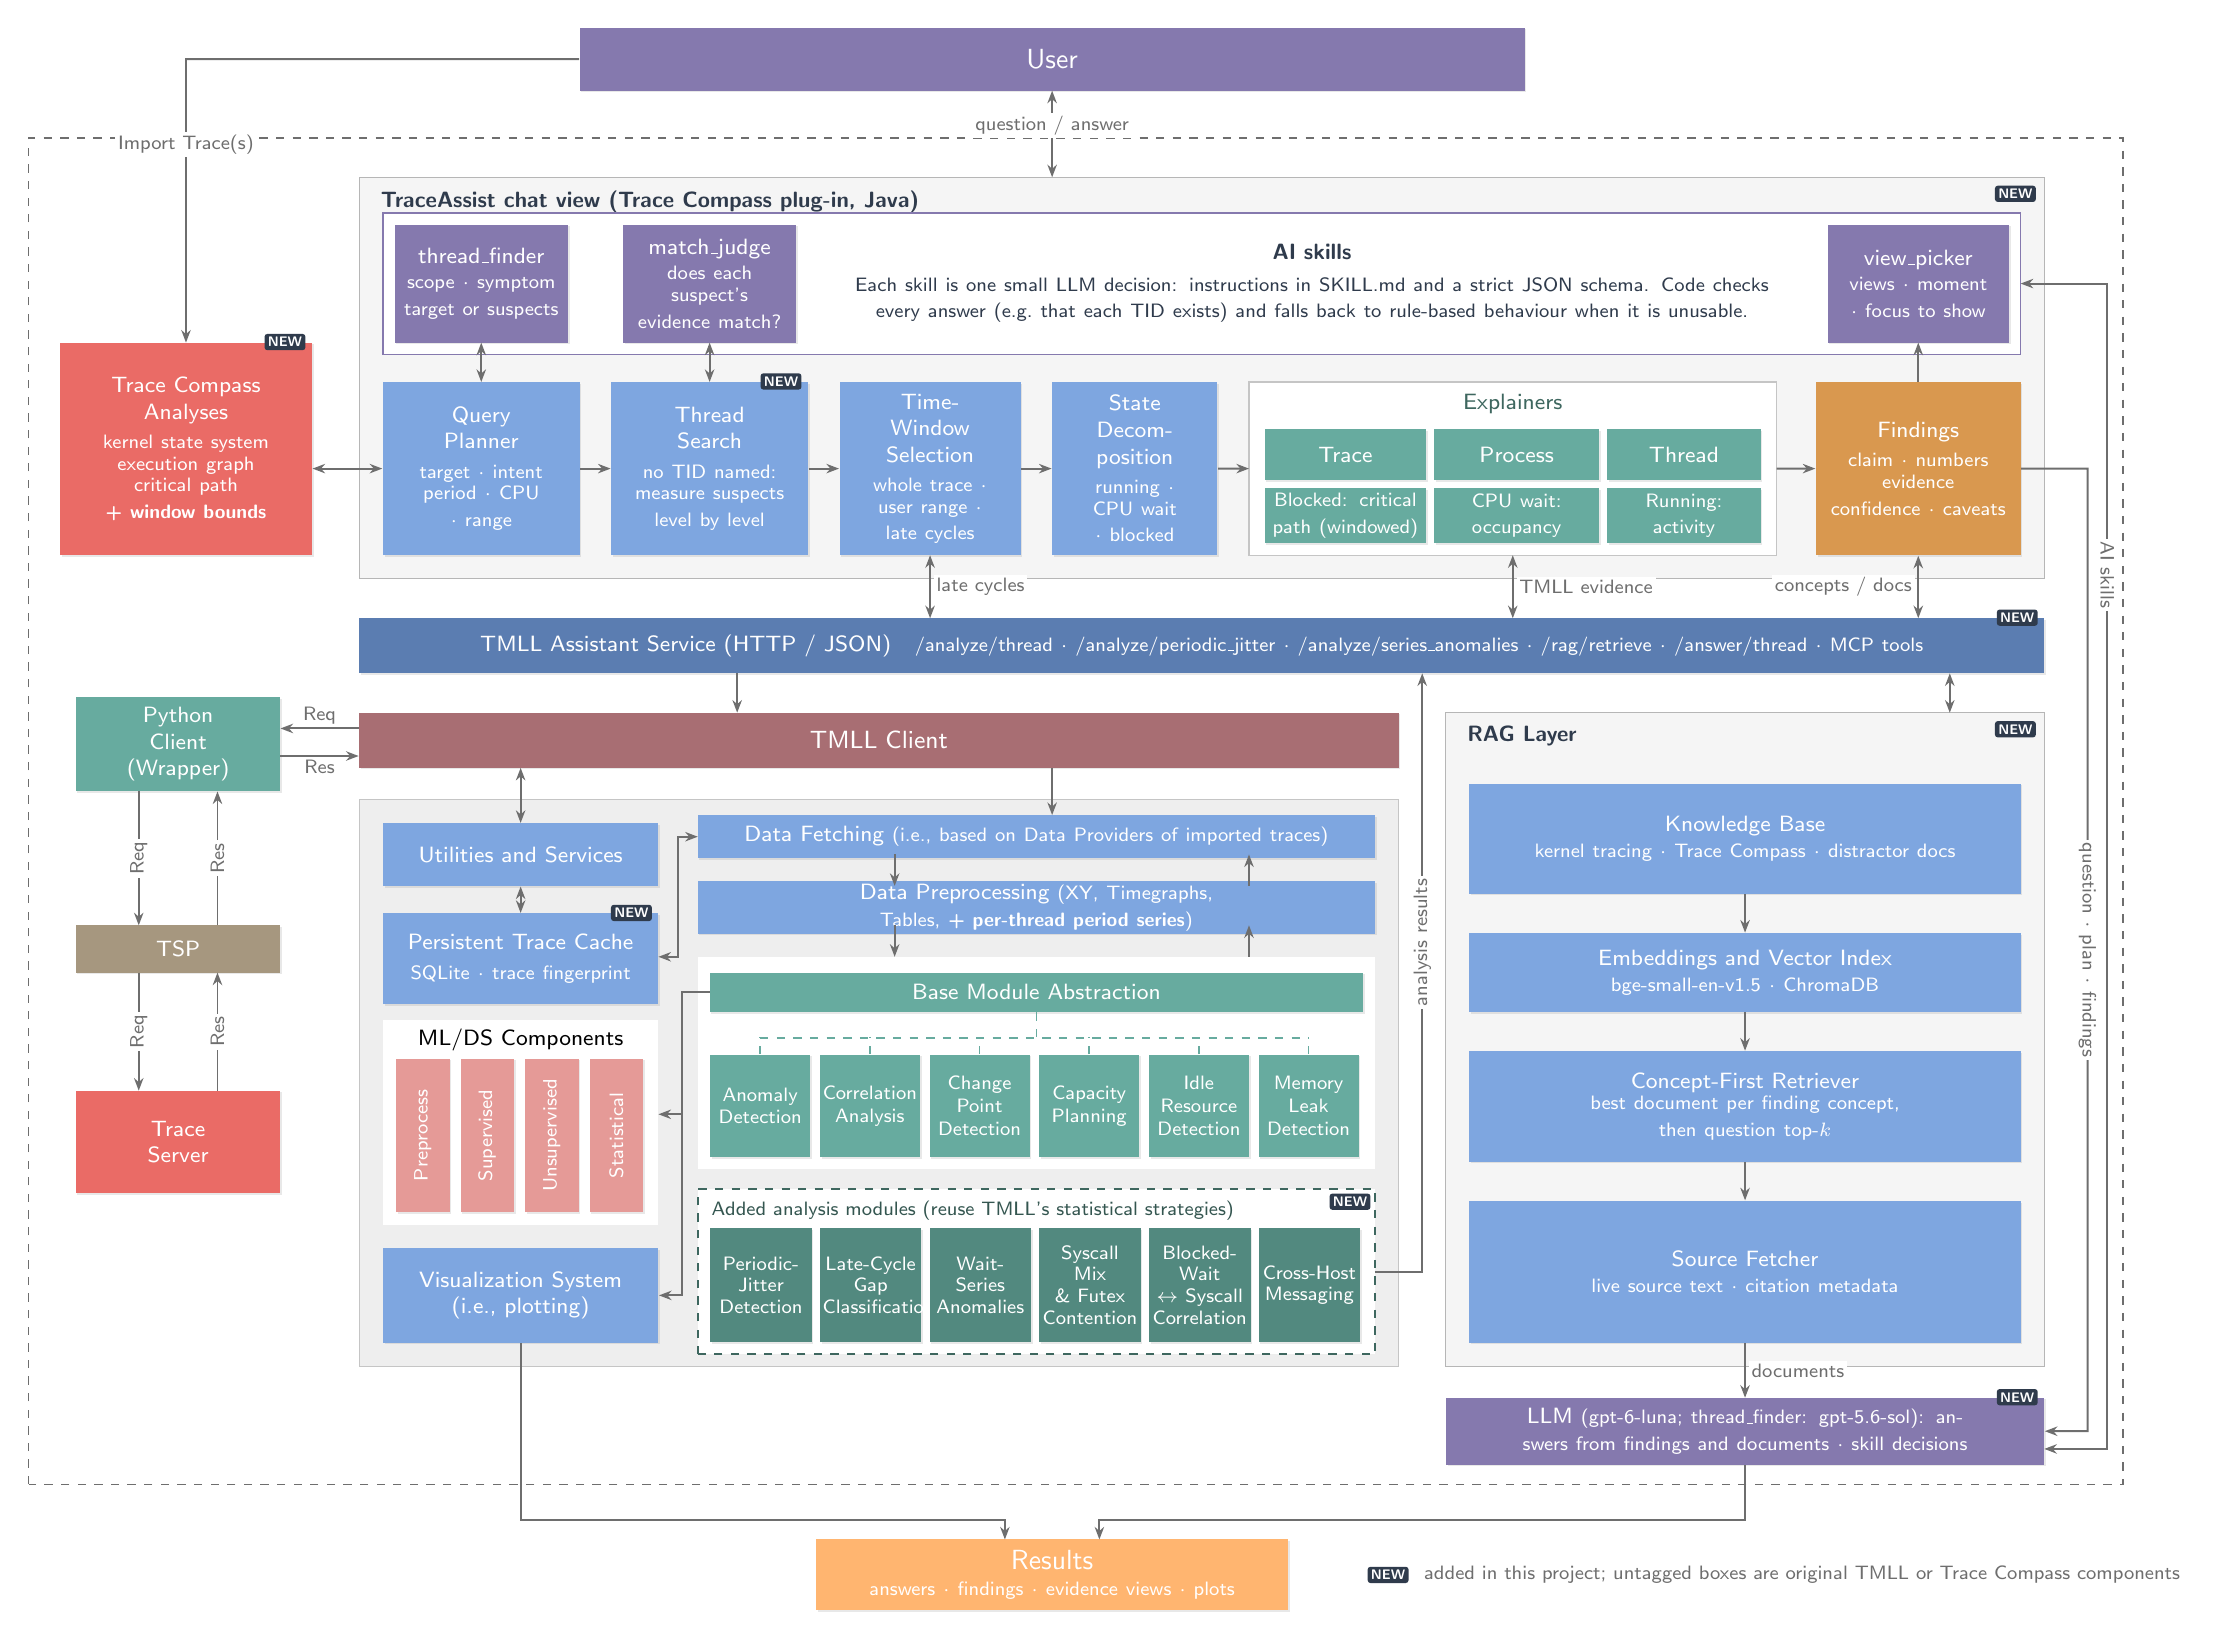
\begin{tikzpicture}[
  font=\fontsize{8}{9.6}\selectfont,
  blk/.style={fill=#1, text=white, align=center, inner sep=1pt,
              drop shadow={opacity=.18, shadow xshift=.6pt, shadow yshift=-.6pt}},
  blk/.default=blue,
  flow/.style={draw=line, line width=.7pt, -{Stealth[length=1.6mm]}},
  both/.style={draw=line, line width=.7pt, {Stealth[length=1.6mm]}-{Stealth[length=1.6mm]}},
  mdash/.style={draw=green, dashed, line width=.6pt},
  lbl/.style={font=\fontsize{7}{8}\selectfont, text=line, fill=white, inner sep=1pt},
  new/.style={fill=badge, text=white, font=\bfseries\fontsize{5.5}{6}\selectfont,
              rounded corners=1pt, inner sep=1.2pt},
]

% \B[colour]{name}{x1}{y1}{x2}{y2}{text}
\newcommand{\B}[7][blue]{%
  \path (#3,#4) coordinate (#2-sw) (#5,#6) coordinate (#2-ne);
  \node[blk=#1, minimum width=#5cm-#3cm, minimum height=#6cm-#4cm,
        text width=#5cm-#3cm-2mm] (#2) at ($(#2-sw)!.5!(#2-ne)$) {#7};}
% NEW tag at the top-right corner of a node.
\newcommand{\NEW}[1]{\node[new, anchor=center] at ([xshift=-3.5mm,yshift=0mm]#1.north east) {NEW};}

% ---- outer boundary ------------------------------------------------------
\draw[line, dashed, line width=.6pt] (0,0.9) rectangle (26.6,18.0);

% ---- user and results ----------------------------------------------------
\B[user]{user}{7}{18.6}{19}{19.4}{\fontsize{10}{12}\selectfont User}
\B[results]{res}{10}{-0.7}{16}{0.2}{\fontsize{10}{12}\selectfont Results\\
  \sub{answers $\cdot$ findings $\cdot$ evidence views $\cdot$ plots}}

% ---- TraceAssist plug-in (Java) -------------------------------------------
\fill[panel!60, draw=line!50] (4.2,12.4) rectangle (25.6,17.5);
\node[anchor=north west, font=\bfseries\fontsize{8}{9.6}\selectfont, text=badge]
  at (4.35,17.45) {TraceAssist chat view (Trace Compass plug-in, Java)};
\node[new, anchor=north east] at (25.5,17.4) {NEW};

\B{plan}{4.5}{12.7}{7.0}{14.9}{Query\\Planner\\[1mm]
  \sub{target $\cdot$ intent\\period $\cdot$ CPU\\$\cdot$ range}}
\B{srch}{7.4}{12.7}{9.9}{14.9}{Thread\\Search\\[1mm]
  \sub{no TID named:\\measure suspects\\level by level}}
\NEW{srch}
\B{win}{10.3}{12.7}{12.6}{14.9}{Time-\\Window\\Selection\\[1mm]
  \sub{whole trace $\cdot$\\user range $\cdot$\\late cycles}}
\B{dec}{13.0}{12.7}{15.1}{14.9}{State\\Decom-\\position\\[1mm]
  \sub{running $\cdot$ CPU wait\\$\cdot$ blocked}}
\fill[white, draw=line!40] (15.5,12.7) rectangle (22.2,14.9);
\node[text=green!60!black, font=\fontsize{8}{9.6}\selectfont] at (18.85,14.62) {Explainers};
\B[green]{ex1}{15.7}{13.65}{17.75}{14.3}{Trace}
\B[green]{ex2}{17.85}{13.65}{19.95}{14.3}{Process}
\B[green]{ex3}{20.05}{13.65}{22.0}{14.3}{Thread}
\B[green]{ex4}{15.7}{12.85}{17.75}{13.55}{\sub{Blocked: critical\\path (windowed)}}
\B[green]{ex5}{17.85}{12.85}{19.95}{13.55}{\sub{CPU wait:\\occupancy}}
\B[green]{ex6}{20.05}{12.85}{22.0}{13.55}{\sub{Running:\\activity}}
\B[findings]{fnd}{22.7}{12.7}{25.3}{14.9}{Findings\\[1mm]
  \sub{claim $\cdot$ numbers\\evidence\\confidence $\cdot$ caveats}}

\draw[flow] (plan) -- (srch);
\draw[flow] (srch) -- (win);
\draw[flow] (win) -- (dec);
\draw[flow] (dec) -- (15.5,13.8);
\draw[flow] (22.2,13.8) -- (fnd);


% ---- AI skills ------------------------------------------------------------
\fill[white, draw=user, line width=.6pt] (4.5,15.25) rectangle (25.3,17.05);
\B[user]{tf}{4.65}{15.4}{6.85}{16.9}{thread\_finder\\[.5mm]
  \sub{scope $\cdot$ symptom\\target or suspects}}
\B[user]{mj}{7.55}{15.4}{9.75}{16.9}{match\_judge\\[.5mm]
  \sub{does each suspect's\\evidence match?}}
\B[user]{vp}{22.85}{15.4}{25.15}{16.9}{view\_picker\\[.5mm]
  \sub{views $\cdot$ moment\\$\cdot$ focus to show}}
\node[text width=11.8cm, align=center, text=badge] at (16.3,16.15)
  {\textbf{AI skills}\\[.6mm]\sub{Each skill is one small LLM decision: instructions in SKILL.md and a strict JSON
  schema. Code checks every answer (e.g.\ that each TID exists) and falls back to rule-based
  behaviour when it is unusable.}};
\draw[both] (5.75,15.4) -- (5.75,14.9);
\draw[both] (8.65,15.4) -- (8.65,14.9);
\draw[flow] (24.0,14.9) -- (24.0,15.4);
\draw[both] (25.3,16.15) -- (26.4,16.15) -- node[lbl, rotate=-90, pos=.25]
  {AI skills} (26.4,1.35) -- (25.6,1.35);

% ---- assistant service ----------------------------------------------------
\B[service]{svc}{4.2}{11.2}{25.6}{11.9}{TMLL Assistant Service (HTTP / JSON)\quad
  \sub{/analyze/thread $\cdot$ /analyze/periodic\_jitter $\cdot$
  /analyze/series\_anomalies $\cdot$ /rag/retrieve $\cdot$ /answer/thread
  $\cdot$ MCP tools}}
\NEW{svc}
\draw[both] (win.south |- 0,12.7) -- node[lbl, right=1pt] {late cycles} (win.south |- 0,11.9);
\draw[both] (18.85,12.7) -- node[lbl, right=1pt] {TMLL evidence} (18.85,11.9);
\draw[both] (fnd.south) -- node[lbl, left=1pt] {concepts / docs} (fnd.south |- 0,11.9);

% ---- TMLL client and core -------------------------------------------------
\B[client]{cli}{4.2}{10.0}{17.4}{10.7}{\fontsize{9}{11}\selectfont TMLL Client}
\draw[flow] (9.0,11.2) -- (9.0,10.7);

\fill[panel, draw=line!40] (4.2,2.4) rectangle (17.4,9.6);

\B{util}{4.5}{8.5}{8.0}{9.3}{Utilities and Services}
\B{cache}{4.5}{7.0}{8.0}{8.15}{Persistent Trace Cache\\[.5mm]
  \sub{SQLite $\cdot$ trace fingerprint}}
\NEW{cache}
\fill[white] (4.5,4.2) rectangle (8.0,6.8);
\node at (6.25,6.55) {ML/DS Components};
\foreach \i/\t in {0/Preprocess,1/Supervised,2/Unsupervised,3/Statistical}
  \node[blk=mlchip, minimum width=.68cm, minimum height=1.95cm, anchor=south west]
    at (4.66+\i*0.82,4.35) {\rotatebox{90}{\fontsize{7}{8}\selectfont\t}};
\B{vis}{4.5}{2.7}{8.0}{3.9}{Visualization System\\(i.e., plotting)}

\B{fetch}{8.5}{8.85}{17.1}{9.4}{Data Fetching \sub{(i.e., based on Data Providers of imported traces)}}
\B{prep}{8.5}{7.95}{17.1}{8.5}{Data Preprocessing \sub{(XY, Timegraphs, Tables, \textbf{+ per-thread period series})}}

\fill[white] (8.5,4.9) rectangle (17.1,7.6);
\B[green]{base}{8.65}{6.9}{16.95}{7.4}{Base Module Abstraction}
\foreach \i/\t in {0/{Anomaly\\Detection},1/{Correlation\\Analysis},
                   2/{Change\\Point\\Detection},3/{Capacity\\Planning},
                   4/{Idle\\Resource\\Detection},5/{Memory\\Leak\\Detection}} {
  \node[blk=green, minimum width=1.25cm, minimum height=1.3cm, text width=1.2cm,
        anchor=south west, font=\fontsize{7}{8.2}\selectfont]
    (m\i) at (8.65+\i*1.393,5.05) {\t};
  \draw[mdash] (m\i.north) -- ++(0,0.22);
}
\draw[mdash] (m0.north |- 0,6.57) -- (m5.north |- 0,6.57);
\draw[mdash] (base.south) -- (base.south |- 0,6.57);

% added modules
\draw[green!60!black, dashed, line width=.7pt, fill=white] (8.5,2.55) rectangle (17.1,4.65);
\node[anchor=north west, text=green!50!black, font=\fontsize{7}{8}\selectfont]
  at (8.55,4.62) {Added analysis modules (reuse TMLL's statistical strategies)};
\node[new, anchor=north east] at (17.05,4.6) {NEW};
\foreach \i/\t in {0/{Periodic-\\Jitter\\Detection},1/{Late-Cycle\\Gap\\Classification},
                   2/{Wait-Series\\Anomalies},3/{Syscall Mix\\\& Futex\\Contention},
                   4/{Blocked-Wait\\$\leftrightarrow$ Syscall\\Correlation},5/{Cross-Host\\Messaging}} {
  \node[blk=green!80!black, minimum width=1.25cm, minimum height=1.45cm, text width=1.22cm,
        anchor=south west, font=\fontsize{6.6}{7.8}\selectfont]
    (n\i) at (8.65+\i*1.393,2.7) {\t};
}

% TMLL-internal flows, as in the original
\draw[both] (6.25,9.3) -- (6.25,10.0);
\draw[flow] (13.0,10.0) -- (13.0,9.4);
\draw[flow] (11.0,8.9) -- (11.0,8.5);
\draw[flow] (15.5,8.5) -- (15.5,8.9);
\draw[both] (cache.north) -- (util.south);
\draw[both] (8.0,7.6) -- (8.25,7.6) |- (8.5,9.125);
\draw[flow] (11.0,8.0) -- (11.0,7.6);
\draw[flow] (15.5,7.6) -- (15.5,8.0);
\draw[flow] (8.65,7.15) -- (8.3,7.15) |- (8.0,5.6);
\draw[flow] (8.3,5.6) |- (vis.east);
% added modules report back to the service
\draw[flow] (17.1,3.6) -- (17.7,3.6) -- node[lbl, rotate=90, pos=.55] {analysis results} (17.7,11.2);

% ---- RAG layer ------------------------------------------------------------
\fill[panel!60, draw=line!50] (18.0,2.4) rectangle (25.6,10.7);
\node[anchor=north west, font=\bfseries\fontsize{8}{9.6}\selectfont, text=badge]
  at (18.15,10.65) {RAG Layer};
\node[new, anchor=north east] at (25.5,10.6) {NEW};
\B{kb}{18.3}{8.4}{25.3}{9.8}{Knowledge Base\\
  \sub{kernel tracing $\cdot$ Trace Compass $\cdot$ distractor docs}}
\B{idx}{18.3}{6.9}{25.3}{7.9}{Embeddings and Vector Index\\
  \sub{bge-small-en-v1.5 $\cdot$ ChromaDB}}
\B{ret}{18.3}{5.0}{25.3}{6.4}{Concept-First Retriever\\
  \sub{best document per finding concept,\\then question top-$k$}}
\B{src}{18.3}{2.7}{25.3}{4.5}{Source Fetcher\\
  \sub{live source text $\cdot$ citation metadata}}
\draw[flow] (kb) -- (idx);
\draw[flow] (idx) -- (ret);
\draw[flow] (ret) -- (src);
\draw[both] (24.4,11.2) -- (24.4,10.7);

% ---- LLM ------------------------------------------------------------------
\B[user]{llm}{18.0}{1.15}{25.6}{2.0}{LLM \sub{(gpt-6-luna; thread\_finder: gpt-5.6-sol): answers from findings and documents $\cdot$ skill decisions}}
\NEW{llm}
\draw[flow] (src.south) -- node[lbl, right=1pt] {documents} (src.south |- 0,2.0);
\draw[flow] (fnd.east) -- (26.15,13.8) -- node[lbl, rotate=-90, pos=.5]
  {question $\cdot$ plan $\cdot$ findings} (26.15,1.575) -- (llm.east);

% ---- left column: data access ---------------------------------------------
\B[server]{tc}{0.4}{12.7}{3.6}{15.4}{Trace Compass\\Analyses\\[1mm]
  \sub{kernel state system\\execution graph\\critical path\\\textbf{+ window bounds}}}
\NEW{tc}
\draw[both] (tc.east |- 0,13.8) -- (plan.west |- 0,13.8);

\B[green]{py}{0.6}{9.7}{3.2}{10.9}{Python\\Client\\(Wrapper)}
\draw[flow] (cli.west |- 0,10.5) -- node[lbl, above=0pt] {\sub{Req}} (3.2,10.5);
\draw[flow] (3.2,10.15) -- node[lbl, below=0pt] {\sub{Res}} (cli.west |- 0,10.15);
\B[tsp]{tsp}{0.6}{7.4}{3.2}{8.0}{TSP}
\B[server]{srv}{0.6}{4.6}{3.2}{5.9}{Trace\\Server}
\draw[flow] (1.4,9.7) -- node[lbl, rotate=90] {\sub{Req}} (1.4,8.0);
\draw[flow] (2.4,8.0) -- node[lbl, rotate=90] {\sub{Res}} (2.4,9.7);
\draw[flow] (1.4,7.4) -- node[lbl, rotate=90] {\sub{Req}} (1.4,5.9);
\draw[flow] (2.4,5.9) -- node[lbl, rotate=90] {\sub{Res}} (2.4,7.4);

% ---- user-facing arrows ---------------------------------------------------
\draw[flow] (user.west) -- (2.0,19.0) -- node[lbl, pos=.3] {Import Trace(s)} (2.0,15.4);
\draw[both] (13.0,18.6) -- node[lbl, pos=.4] {question / answer} (13.0,17.5);
\draw[flow] (vis.south) -- (6.25,0.45) -- (12.4,0.45) -- (12.4,0.2);
\draw[flow] (llm.south) -- (21.8,0.45) -- (13.6,0.45) -- (13.6,0.2);

% ---- legend ---------------------------------------------------------------
\node[new, anchor=west] at (17.0,-0.25) {NEW};
\node[anchor=west, font=\fontsize{7}{8}\selectfont, text=line] at (17.6,-0.25)
  {added in this project; untagged boxes are original TMLL or Trace Compass components};
\end{tikzpicture}
\end{document}
